% !TeX root = ..

\section{
  Вариант <<жадного>> эвристического алгоритма
}
\label{sect:5.6}
\setcounter{equation}{0}

В задачах раскроя количество контуров нередко превышает несколько сотен.
Для решения таких задач предлагается использовать эвристические методы.
Кроме того,
в задачах раскроя важную роль играют тепловые и геометрические ограничения.
Несоблюдение этих ограничений делает бессмысленной
оптимизацию длины пути.

Рассмотрим один из подходов к построению эвристического алгоритма для решения
задач большой размерности при наличии упомянутых ограничений.
В данном подходе оптимизирующие вставки не используются.

В качестве $X$
предполагается заданным достаточно большой прямоугольник на плоскости,
соответствующий листу металла.
Процедура раскроя полагается выполненной.
В результате в пределах $X$ размещены контуры деталей,
подлежащие резке по некоторым эквидистантам в виде замкнутых кривых.
С внешней по отношению к деталям стороны вблизи каждой эквидистанты
размещены конечные множества --- мегаполисы.
Точки мегаполисов группируются в упорядоченный пары.
Элементами каждой такой упорядоченной пары являются точка
врезки и точка выключения инструмента.
Каждой такой упорядоченной паре сопоставляется также точка на эквидистанте,
определяющая начало и завершение реза соответствующего контура.

Как и в предыдущих разделах,
фиксируются скорости холостого хода и реза
$V_i>0$ и $V_c>0$ соответственно.
Значения функции $\mathbf{c}$
определяются соответствующим временем внешних перемещений.
При этом точка
$x^0$ задается в виде начала координат
$x^0=(0,0)$.
Функция $\mathbf{c}$
та же, что и в (\ref{ExtPrice}).
Функция $f$ та же, что и в
(\ref{TerminalPrice}).

Перейдем к рассмотрению функций стоимости внутренних работ
$c_1,\,\dots,c_N$,
в которых используется зависимость от списка заданий.

Пусть
$j\in \overline{1,N}$,
$z=(x,y)\in \mathbb{M}_j$ и
$u=u(z)$ --- отвечающая паре $z$ точка на $j$-й эквидистанте.
Кроме того, обозначим через
$\tilde{D}$,
$\tilde{D}\stackrel{\triangle}{=}\{0;1\}$,
множество, соответствующее возможным направлениям реза,
причем $1$
определяет направление реза по часовой стрелке,
$0$ --- против часовой стрелки.
Скорость реза здесь также совпадает с $V_c, V_c>0$.

Важным ограничением при резке металла является требование достаточного
количества металла возле завершающего участка реза.
Рассеивание тепла особенно важно на финишном участке.
В свете этого ограничения большую значимость приобретает направление реза.
Дело в том,
что при резе в разных направлениях участок завершения реза
также оказывается с разных сторон от точки начала реза.
При этом ситуация с количеством металла
с этих разных сторон может сильно различаться.

Условимся относительно следующих обозначений,
применяемых ниже в целях формализации
содержательных понятий <<много металла>> и <<мало металла>>.
Итак, если
$j\in \overline{1,N}$,
$z\in \mathbb{M}_j$,
$d\in \tilde{D}$ и
$\mathbb{K}\in \mathcal{P}(\overline{1,N}\setminus \{j\})$,
то через
$S_1(j,z,d,\mathbb{K})$ обозначаем площадь пересечения заданной
области вокруг участка завершения реза и области имеющегося металла,
а через
$S_2(j,z,d,\mathbb{K})$ --- площадь пересечения упомянутой областии пустот,
образовавшихся после вырезания контуров с номерами из $\mathbb{K}$,
а также внешнего пространства, выходящего за края листа.
Под областью возле участка завершения реза подразумевается геометрическая фигура,
лежащая вне детали, и такая,
что расстояние от любой ее точки до ближайшей точки участка
завершения реза не превышает заданной величины
(см. рис. \ref{FinishCutArea}).

Пусть
$\tilde{K}, \tilde{K}\subset \overline{1,N}\setminus \{j\}$
--- множество номеров вырезанных к текущему моменту контуров,
и $k\in \tilde{K}$.
На рис. \ref{FinishCutArea}
изображены два варианта реза ---
по часовой стрелке и против часовой стрелки.
На рисунке область завершения реза пересекается только с вырезанным
контуром с номером $k$.

Стоимость внутренних работ
при $K=\overline{1,N}\setminus \tilde{K}$
по вырезанию контура с номером $j,j\in \overline{1,N},$
при использовании пары $z$ точек врезки и выключения инструмента,
$z\in \mathbb{M}_j$,
в направлении $d,d\in \tilde{D},$ при условии,
что к настоящему моменту уже вырезаны контура с номерами из
$\tilde{K},\tilde{K}\subset \overline{1,N}\setminus \{j\}$,
будет вычисляться следующим образом:
\begin{equation}\label{IntPrice}
  \begin{array}{c}
  c_j(z,d,K)=\frac{\rho(\mbox{pr}_1(z),u(z))}{V_c}+
  \frac{\rho(u(z),\mbox{pr}_2(z))}{V_c}+\\
  +\frac{S_2(j,z,d,\overline{1,N}\setminus K)}{S_1(j,z,d,\overline{1,N}\setminus K)+
  S_2(j,z,d,\overline{1,N}\setminus K)}\cdot\tilde{P}
  .
  \end{array}
\end{equation}

Коэффициент $\tilde{P}$
определяет влияние штрафа в зависимости от расположения финишной области реза.
Если
$\tilde{P}=0$,
то расположение финишной области никак не
сказывается на стоимости маршрута.
Если $\tilde{P}$
есть большая величина,
то основная часть стоимости внутренних
работ в основном определяется вышеупомянутым штрафом,
а не временем реза на подходе к контуру.

\begin{figure}[H]
  \center
  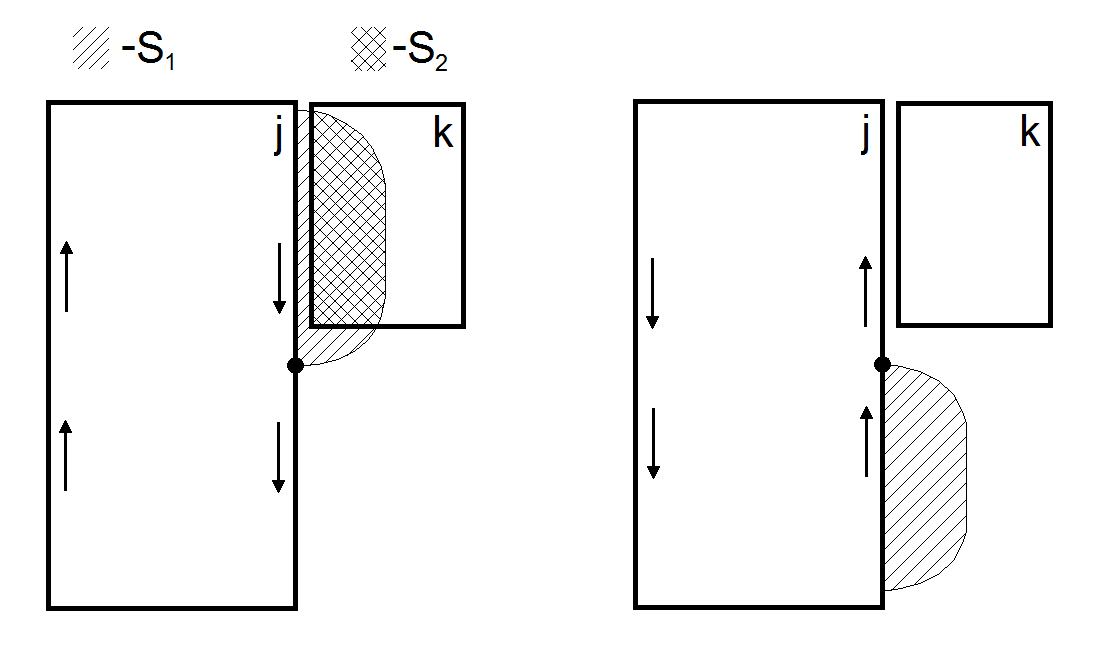
\includegraphics[width=0.9\textwidth]{CutFinishArea.png}
  \caption{
    Область металла возле участка завершения реза;
    резка против часовой стрелки здесь более предпочтительна
  }
  \label{FinishCutArea}
\end{figure}

Эвристический алгоритм показан в виде ряда шагов.
Изначально считается, что маршрут пуст.
Далее к нему на каждом шаге добавляется номер одного мегаполиса.

\begin{enumerate}
  \item
  Находим мегаполис с номером $i$, $i\in \overline{1,N},$
  для которого
  $i\neq \mbox{pr}_2(z)$ $\forall z\in \mathbf{K}$,
  и упорядоченную пару
  $(x,y)\in \mathbb{M}_i$,
  а также $d\in \tilde{D}$,
  обеспечивающие минимум значения
  $\mathbf{c}(x^0,x)+c_i((x,y),d,\overline{1,N})$.
  Добавляем мегаполис $M_i$ в маршрут,
  а пару точек $(x,y)$ --- на трассу.
  Отмечаем мегаполис $M_i$ как посещенный с направлением обхода $d$.

  \item
  Через $V$, $V\subset \overline{1,N},$
  обозначим множество номеров уже посещенных мегаполисов.
  Пусть $j,j\in V$
  является номером последнего мегаполиса частичного маршрута,
  а $(x,y)\in \mathbb{M}_j$ его пара точек входа и выхода.
  Далее находим номер мегаполиса
  $k,k\in I(\overline{1,N}\setminus V)$,
  а также
  $(\tilde{x},\tilde{y})\in \mathbb{M}_k$ и $d\in \tilde{D}$,
  которые обеспечивают минимальное значение выражения
  $\mathbf{c}(y,\tilde{x})+c_k((\tilde{x};\tilde{y}),d,\overline{1,N}\setminus V)$.
  Добавляем мегаполис $M_k$ в маршрут, а пару точек $(\tilde{x},\tilde{y})$
  --- на трассу.
  Отмечаем мегаполис с номером $k$ как посещенный с направлением
  обхода $d$.

  \item
  Выполняем шаг 2 до тех пор,
  пока весь маршрут не будет построен.
\end{enumerate}

Данный алгоритм позволяет получить некоторое допустимое решение.
Так как алгоритм <<жадный>>,
то при его реализации значительный поиск глобального экстремума не производится.
Алгоритм может выдать некоторый локальный экстремум.
В целях улучшения результата в данной работе предлагается вариант
многократного выполнения алгоритма с запретами определенных перемещений,
обеспечивающими возможность получения всякий раз новых
маршрута и трассы.
Данные запреты осуществляются посредством изменения функций
стоимости $c_1,\,\dots,c_N$.
Именно для заданного мегаполиса значение этой функции
принимает очень большую величину,
если он попадает в заранее оговоренную позицию маршрута.
Следовательно, алгоритм будет избегать посещения упомянутого мегаполиса
в данной выбранной позиции.

Для реализации этого подхода вводится специальная матрица
$D$ коррекции стоимостей внутренних работ:
$D_{i,j}\in \{0;1\}$, $i\in \overline{1,N}$, $j\in \overline{1,N}$.
Если $D_{i,j}=1$, то
$$
  c_i(h,d,K)=1000000\;\; \forall h\in \mathbb{M}_i,\;\;
  \forall d\in \tilde{D},\;\;\forall K\in \mathcal{P}(\overline{1,N}\setminus \{i\})
$$
при условии, что мегаполис с номером $i$ помещен на маршруте в позицию $j$.
Если же $D_{i,j}=0$,
то оценка внутренних работ вычисляется обычным способом,
см. (\ref{IntPrice}).
Данный способ вычисления внутренних стоимостей используется
только во время построения маршрута и трассы,
для их оценки он не используется.

Работа итерационного алгоритма определяется двумя параметрами.
$N_1$ определяет общее количество итераций,
$N_2$ определяет количество итераций в одном цикле.
Смысл цикла итераций заключается в постепенном добавлении новых коррекций
(единиц в матрице $D$)
к уже существующим.
После завершения цикла все значения матрицы $D$ сбрасываются в ноль.
Далее итерационный метод использования алгоритма приводится в виде ряда шагов.

\begin{enumerate}
  \item
  Выполнение алгоритма без каких-либо коррекций.
  \item
  Выбираем случайным образом позицию
  $i,i\in \overline{1,N}$ на маршруте.
  Пусть в данной позиции располагается мегаполис с номером
  $j$, $j\in \overline{1,N}$.
  Принимаем $D_{j,i}=1$.
  \item
  Выполняем описанный ранее алгоритм.
  Вычисляем оценку маршрута и трассы без коррекций.
  Если значение оценки улучшилось, то запоминаем данное значение,
  а также полученные маршрут, трассу и направления обхода мегаполисов.
  \item
  Выполняем шаги 2 и 3 $N_2-1$ раз
  ($N_2-2$ раза для первого цикла итераций,
  так как в самом начале был произведен счет без коррекций).
  \item
  Обнуляем матрицу $D$.
  \item
  Выполняем шаги 2 -- 5,
  пока общее количество итераций не достигнет $N_1$.
  \item
  Выбираем лучший результат,
  а также соответствующие ему маршрут, трассу
  и направления обхода мегаполисов.
\end{enumerate}

\paragraph*{Пример 1.}

Скорость холостого хода $V_i=500$ мм/с,
скорость реза $V_c=10$~мм/с.
Длина финишного участка реза равна 150 мм,
ширина области завершения реза 50 мм.
Параметры итерационного метода в обоих примерах
$N_1=100$, $N_2=10$,
коэффициент штрафа для внутренних работ
$\tilde{P}=1\,000\,000$.
Количество контуров $N=170$,
количество адресных пар $|\mathbf{K}|=80$.

Результат счета 532.99,
результат на первой итерации 556.15.
Время счета 8 мин 23 с.
Маршрут и трасса показаны на рис. \ref{Sample1Heuristic}.

\paragraph*{Пример 2.}

Скорость холостого хода $V_i=500$ мм/с,
скорость реза $V_c=10$~мм/с.
Длина финишного участка реза равна 150 мм,
ширина области завершения реза 50 мм.
Параметры итерационного метода в обоих примерах
$N_1=100$, $N_2=10$,
коэффициент штрафа для внутренних работ
$\tilde{P}=1\,000\,000$.
Количество контуров $N=201$,
количество адресных пар $|\mathbf{K}|=56$.

Результат счета 2\,255\,679.293,
результат без учета штрафов 531.631
(совпадает со значением на первой итерации).
Время счета 1 мин 40 с.
Маршрут и трасса показаны на рис. \ref{Sample2Heuristic}.

\begin{figure}[H]
  \centering
  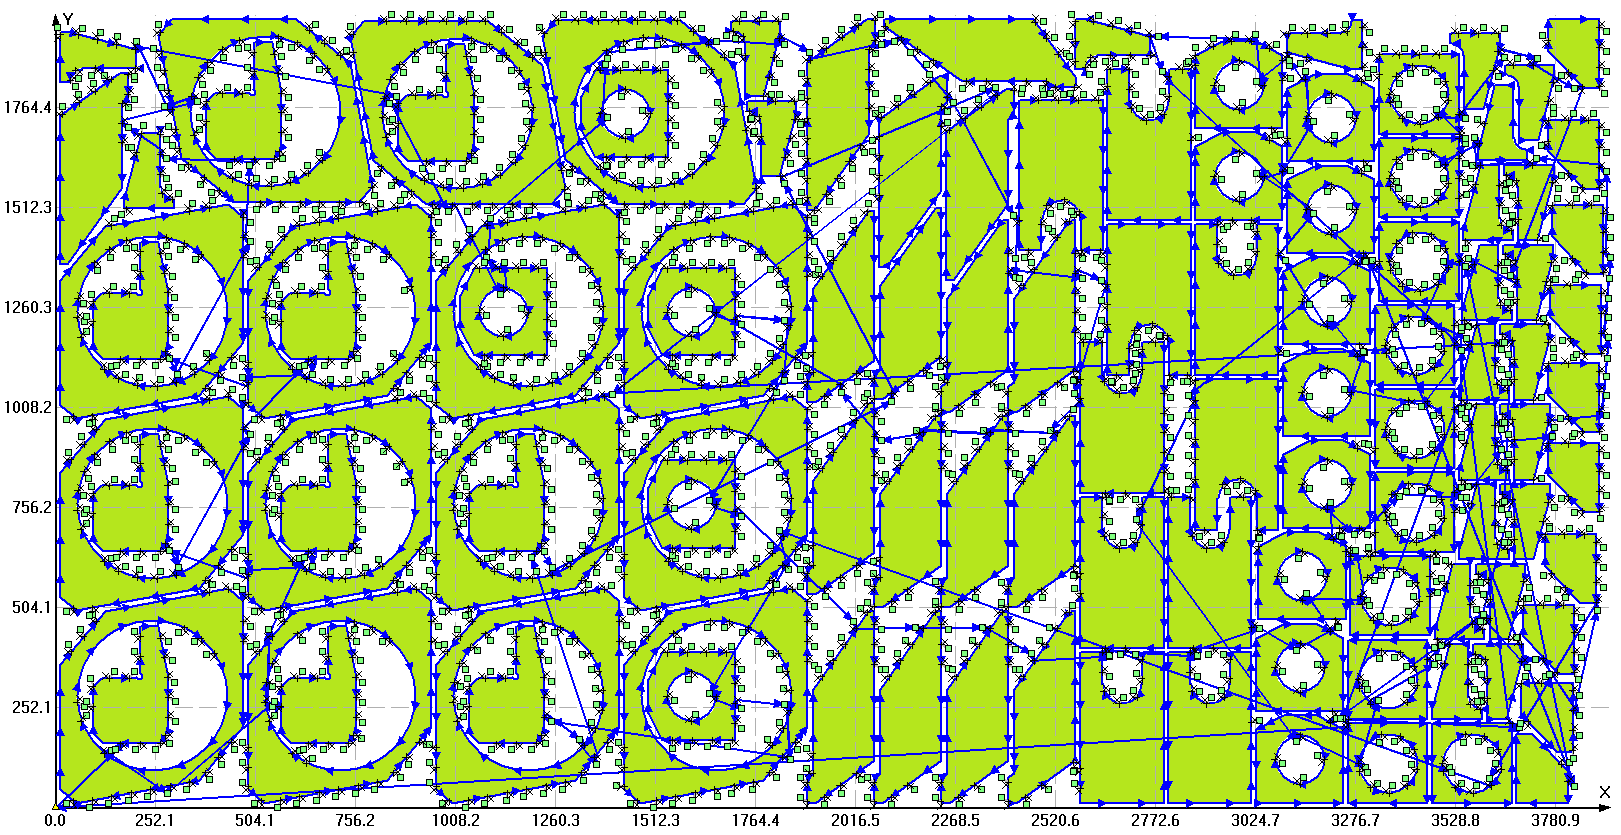
\includegraphics[width=0.9\textwidth]{route_170_approximate_CA.png}
  \caption{
    Маршрут и трасса обхода множеств \\
    (Пример 1. Эвристический алгоритм)
    }
  \label{Sample1Heuristic}
\end{figure}

\begin{figure}[H]
  \centering
  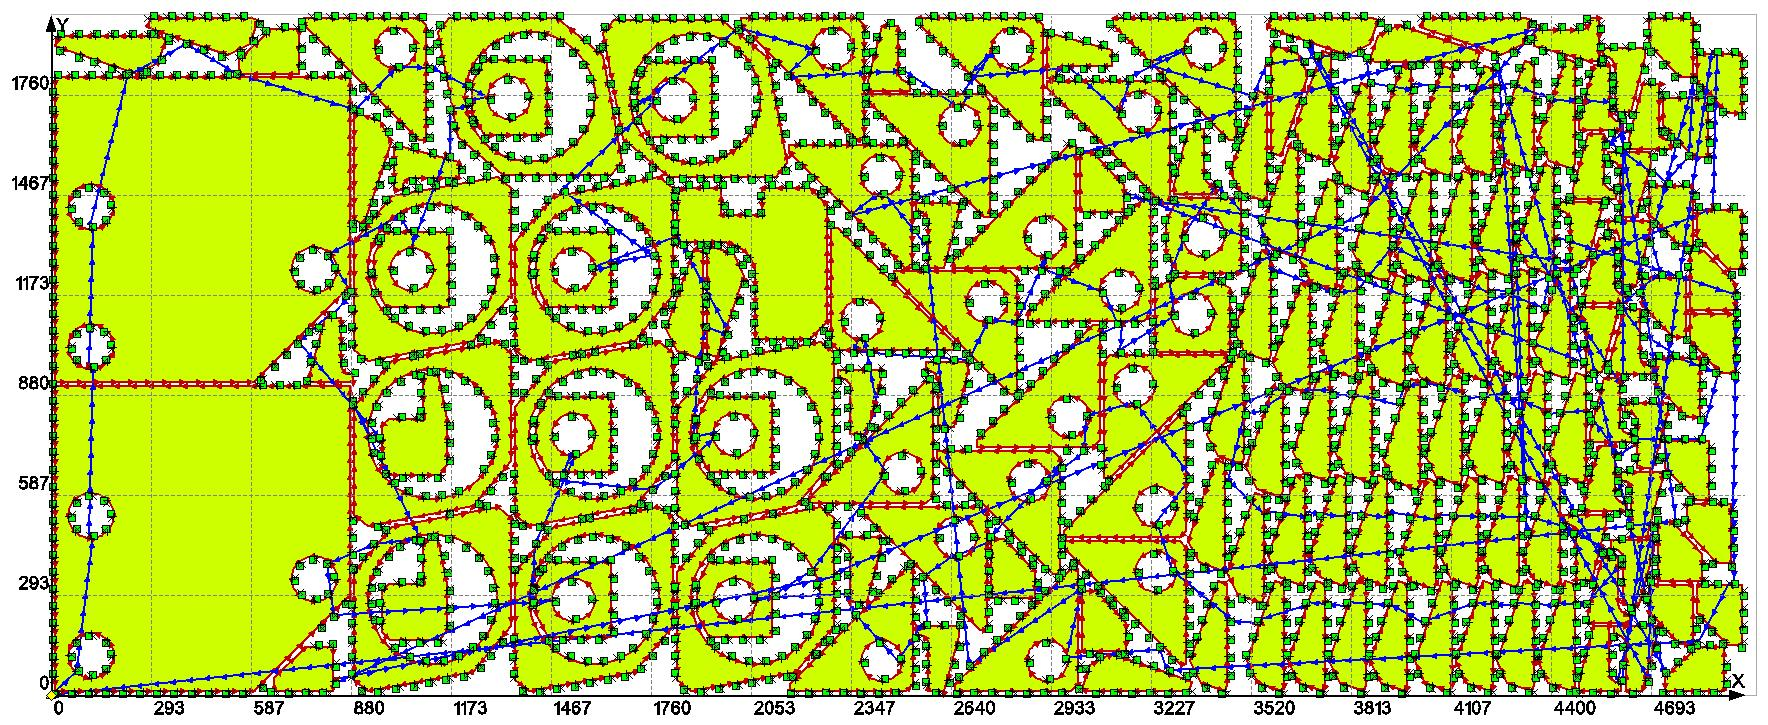
\includegraphics[width=0.9\textwidth]{Sample_201_sets_approximate.png}
  \caption{
    Маршрут и трасса обхода множеств\\
    (Пример 2. Эвристический алгоритм)
    }
  \label{Sample2Heuristic}
\end{figure}

В данном случае максимальный штраф составил 387\,001.
Учитывая тот факт, что максимально возможный штраф имеет значение 1\,000\,000
(если вся область завершения реза приходится на пустоты в металле),
то можно сделать вывод, что 38~\% области
завершения реза пришлось на пустоты в металле для данного контура.
Такой результат может быть естественным следствием очень плотной компоновки деталей
и, в принципе, вряд ли является критичным.

\paragraph*{Пример 3.}

Скорость холостого хода $V_i=500$ мм/с,
скорость реза $V_c=10$~мм/с.
Длина финишного участка реза равна 150 мм,
ширина области завершения реза 50~мм.
Решение получено с использованием метода динамического программирования
и эвристического итерационного алгоритма.
Коэффициент штрафа для внутренних работ
$\tilde{P}=1\,000\,000$.
В случае эвристического алгоритма параметры итерационного
метода имели следующие значения
$N_1=10\,000$,
$N_2=10$.
Количество контуров $N=27$,
количество адресных пар $|\mathbf{K}|=12$.

Результат счета методом ДП 62.815,
результат без учета штрафов 62,815.
Время счета 7 мин 25 с.
Маршрут и трасса показаны на рис. \ref{Sample3DP}.

Результат счета эвристическим итерационным методом 243\,112.454,
результат без учета штрафов 68.495
(для первой итерации 243\,113.235 и 69.276
соответственно).
Маршрут и трасса показаны на рис. \ref{Sample3Heuristic}.

Максимальный из штрафов составил 176\,823.72.
Можно сделать вывод, что 17~\% области завершения реза пришлось на пустоты для
данного контура, что достаточно неплохо.
Время счета 25 с.

Особенность метода ДП состоит в том,
что размерность решаемых с его использованием примеров
ограничена приблизительно четырьмя десятками контуров.
В принципе, такие задачи уже представляют практический интерес
(возможны раскрои такой размерности).
Кроме того, метод ДП может использоваться для грубой оценки
приведенного эвристического алгоритма.
Именно, предлагается выполнить вычисления на нескольких десятках
примеров эвристическим методом и методом ДП,
после чего сравнить результаты.
Ниже приведены результаты такого сравнения.

Количество примеров равно 25.
Высота области, занимаемой контурами,
приблизительно равна одному метру.
Ширина колеблется в пределах от одного до двух метров.
Матрицы, используемая для построения значений функций стоимости,
имеют 1500 столбцов и 700 строк.

Скорость холостого хода $V_i=500$ мм/с,
скорость реза $V_c=10$ мм/с.
Длина финишного участка реза равна 100 мм,
ширина области завершения реза 25 мм.
Параметры итерационного метода во всех примерах
$N_1=100$, $N_2=10$,
коэффициент штрафа для внутренних работ
$\tilde{P}=1000$.
Количество контуров в каждом из примеров
$N=20$.
Количество адресных пар $|\mathbf{K}|$ принимало значение от 2 до 22.
Далее через
$T_h$ будем обозначать значение критерия для эвристического алгоритма,
а через $T_{DP}$ -- для метода ДП.
Результаты вычислительного эксперимента
сведены в табл.~\ref{28lines}.

\begin{figure}[p]
  \centering
  \subfigure[]{
    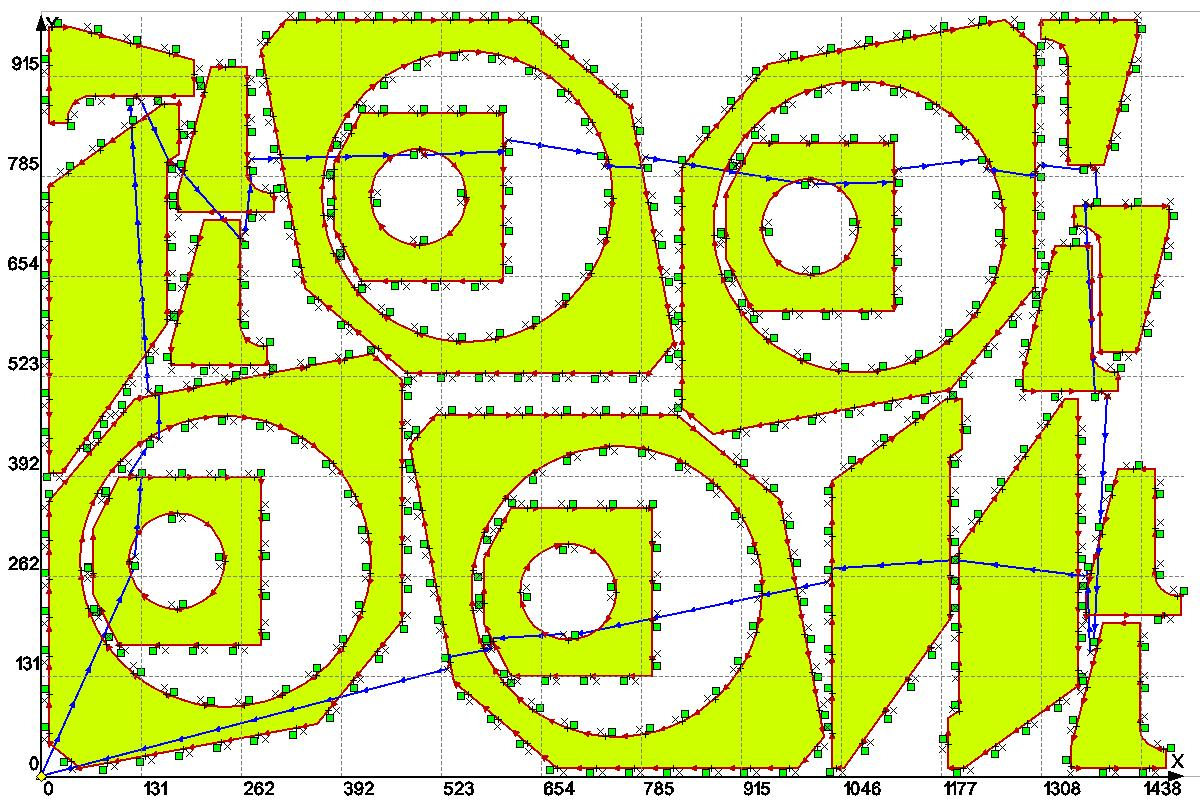
\includegraphics[width=0.9\textwidth]{Sample_27_sets_DP.png}
    \label{Sample3DP}
  }
  \subfigure[]{
    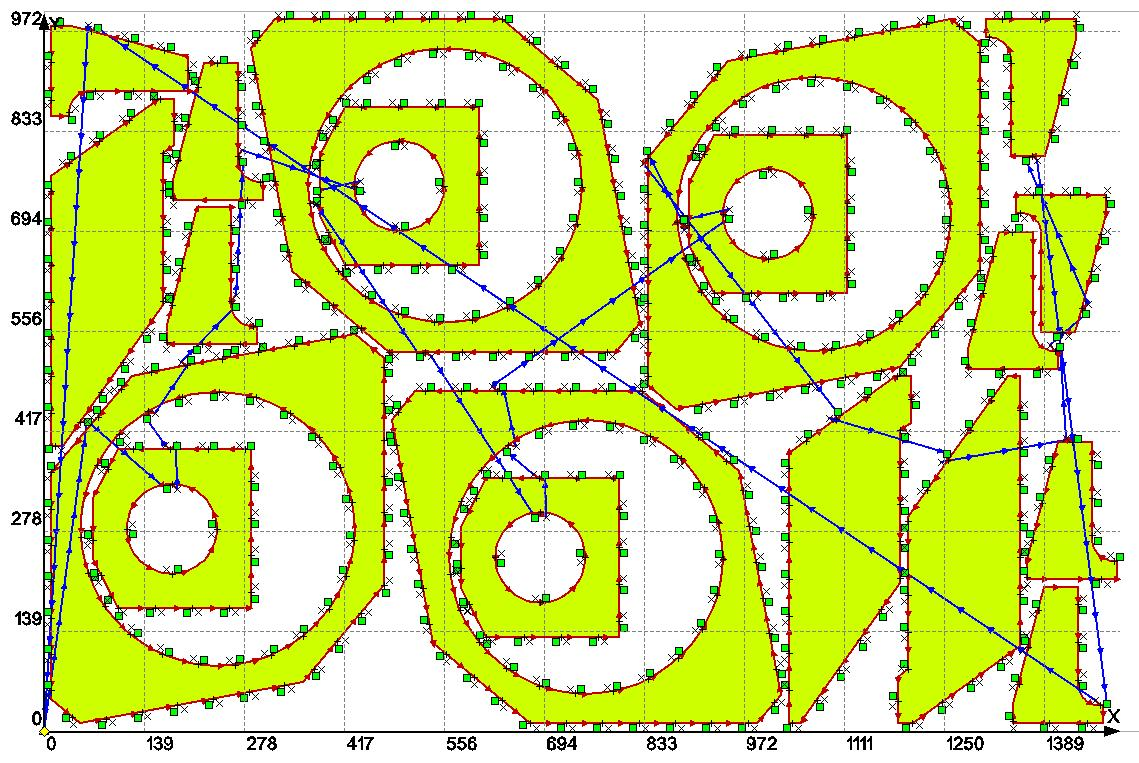
\includegraphics[width=0.9\textwidth]{Sample_27_sets_approximate.png}
    \label{Sample3Heuristic}
  }
  \caption{
    Маршрут и трасса обхода множеств:\\
    {\it а} -- ДП;
    {\it б} -- Эвристический алгоритм
    }
\end{figure}

\begin{table}[p]
  \caption{Сравнение результатов работы эвристического алгоритма и~ДП}
  \label{28lines}
  \centering
  \begin{tabular}{c *{2}{|c}}
    Пример & $T_h$ & $T_{DP}$ \\
    \hline
     4  & 71.41 & 66.42 \\
     5  & 372.35 & 136.89 \\
     6  & 67.40 & 66.30 \\
     7  & 263.41 & 66.68 \\
     8  & 64.29 & 63.18 \\
     9  & 70.26 & 67.60 \\
     10 & 64.41 & 62.87 \\
     11 & 68.16 & 67.07 \\
     12 & 139.32 & 136.64 \\
     13 & 68.30 & 66.58 \\
     14 & 114.10 & 65.53 \\
     15 & 70.10 & 67.85 \\
     16 & 69.00 & 66.61 \\
     17 & 68.06 & 66.83 \\
     18 & 66.39 & 64.94 \\
     19 & 69.83 & 68.35 \\
     20 & 69.69 & 66.46 \\
     21 & 68.28 & 66.38 \\
     22 & 171.85 & 65.25 \\
     23 & 68.11 & 66.39 \\
     24 & 308.90 & 135.72 \\
     25 & 69.05 & 67.29 \\
     26 & 68.27 & 66.16 \\
     27 & 221.97 & 66.86 \\
     28 & 68.78 & 66.92 \\
    \hline
  \end{tabular}
\end{table}

\subsubsection*{Выводы}

Сравнивая результаты работы эвристического алгоритма и
алгоритма на основе ДП можно отметить следующие моменты.
В трех примерах из 24 найти точное решение без штрафов не удалось.
Напомним, штрафы возникают,
если область вокруг участка завершения реза пересекается с отверстиями в металле
или выходит за края листа.
Причем в одном случае эвристический алгоритм дал близкий к оптимальному результат,
а в двух других случаях штраф был заметно больше, чем в случае с ДП.
Еще в четырех примерах эвристический алгоритм дал
результат со штрафами.

Максимальное значение критерия для одного из примеров
для эвристического алгоритма равно 372.35.
Оптимальный результат для этого примера 136.89
(есть штрафы, величина которых составляет 68.95).
Для ДП стоимость маршрута без учета штрафов 68.09,
для эвристического алгоритма --- 68.95.
Таким образом, без учета штрафов результаты счета очень близки.
В случае с эвристическим алгоритмом величина штрафа равна 303.4.
Напомним, что коэффициент штрафа для внутренних работ $\tilde{P}=1000$.
Если вся область вокруг участка завершения реза попадает на пустоты,
то штраф для данного контура будет равен 1000.
Даже в том случае, если вся величина штрафа 303.4 попала на один контур,
менее трети области вокруг участка завершения реза пересекается с пустотами в металле.
Такой результат представляется вполне приемлемым с практической точки зрения.

Итак, данный эвристический алгоритм представляется весьма эффективным.
Что касается алгоритма на основе ДП --- он дает оптимальный результат,
что исключительно важно,
но размерость решаемых этим методом примеров лежит в пределах четырех десятков контуров.
Данное обстоятельство накладывает значительные ограничения на практическое его использование.
